\documentclass[a4paper]{arrowhead}

\usepackage[yyyymmdd]{datetime}
\usepackage{etoolbox}
\usepackage[utf8]{inputenc}
\usepackage{multirow}
\usepackage[]{url}

\renewcommand{\dateseparator}{-}

%% Special references
\newcommand{\fref}[1]{{\textcolor{ArrowheadBlue}{\hyperref[sec:functions:#1]{#1}}}}
\newcommand{\mref}[1]{{\textcolor{ArrowheadPurple}{\hyperref[sec:model:#1]{#1}}}}
\newcommand{\pdef}[1]{{\textcolor{ArrowheadGrey}{#1\label{sec:model:primitives:#1}\label{sec:model:primitives:#1s}\label{sec:model:primitives:#1es}}}}
\newcommand{\pref}[1]{{\textcolor{ArrowheadGrey}{\hyperref[sec:model:primitives:#1]{#1}}}}

\newrobustcmd\fsubsection[3]{
  \addtocounter{subsection}{1}
  \addcontentsline{toc}{subsection}{\protect\numberline{\thesubsection}function \textcolor{ArrowheadBlue}{#1}}
  \renewcommand*{\do}[1]{\rref{##1},\ }
  \subsection*{
    \thesubsection\quad
    operation
    \textcolor{ArrowheadBlue}{#1}
    (\notblank{#2}{\mref{#2}}{})
    \notblank{#3}{: \mref{#3}}{}
  }
  \label{sec:functions:#1}
}
\newrobustcmd\msubsection[2]{
  \addtocounter{subsection}{1}
  \addcontentsline{toc}{subsection}{\protect\numberline{\thesubsection}#1 \textcolor{ArrowheadPurple}{#2}}
  \subsection*{\thesubsection\quad#1 \textcolor{ArrowheadPurple}{#2}}
  \label{sec:model:#2} \label{sec:model:#2s} \label{sec:model:#2es}
}
%%


\begin{document}

%% Arrowhead Document Properties
\ArrowheadTitle{Fundational principles} % XXX = SystemName e.g. Service Registry HTTP/TLS/JSON}
\ArrowheadType{Eclipse Arrowhead}
\ArrowheadTypeShort{Foundational principles}
\ArrowheadVersion{4.6.1} % Arrowhead version X.Y.Z, e..g. 4.4.1
\ArrowheadDate{\today}
\ArrowheadAuthor{Jerker Delsing} % Corresponding author e.g. Jerker Delsing
\ArrowheadStatus{DRAFT} % e..g. RELEASE, RELEASE CONDIDATE, PROTOTYPE
\ArrowheadContact{jerker.delsing@ltu.se} % Email of corresponding author
\ArrowheadFooter{\href{www.arrowhead.eu}{www.arrowhead.eu}}
\ArrowheadSetup
%%

%% Front Page
\begin{center}
  \vspace*{1cm}
  \huge{\arrowtitle}

  \vspace*{0.2cm}
  \LARGE{\arrowtype}
  \vspace*{1cm}

  \begin{figure*}[h!]
    \centering
    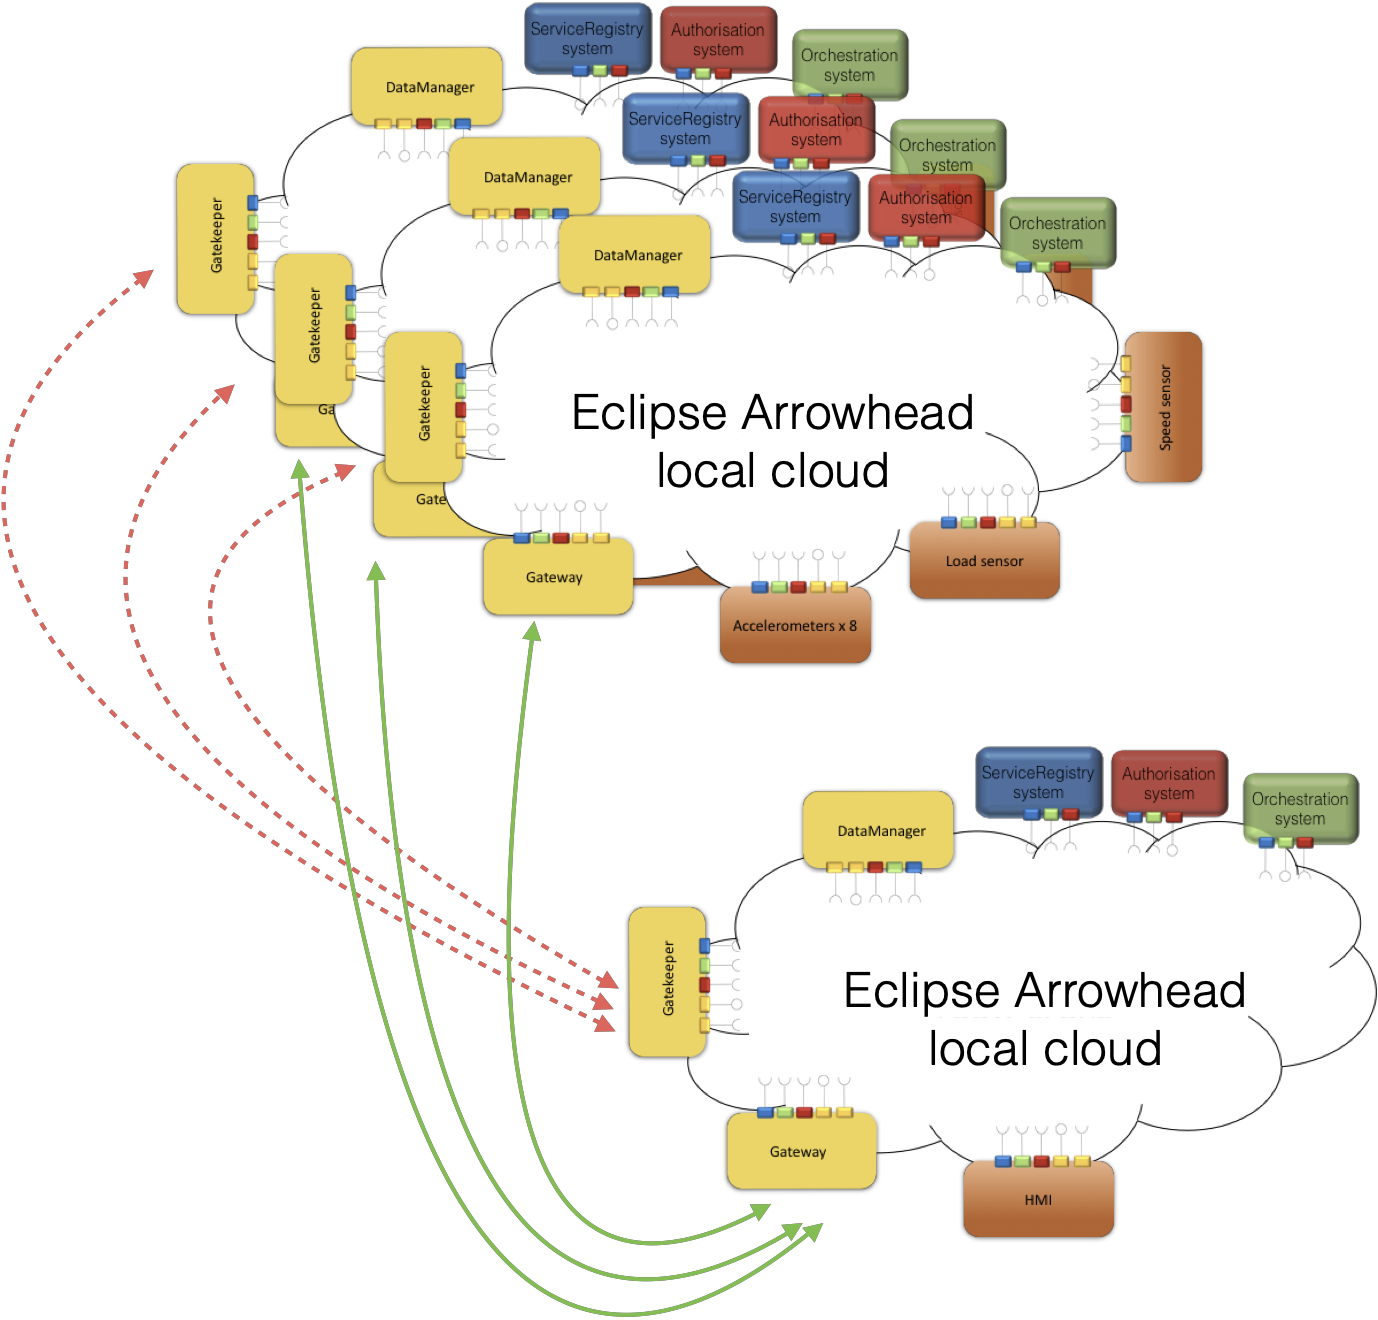
\includegraphics[]{figures/Arrowhead_Local_Clouds}
  \end{figure*}
  
  %\Large{Service ID: \textit{"\arrowid"}}
  \vspace*{\fill}

  % Front Page Image
  %\includegraphics{figures/TODO}

  \vspace*{1cm}
  \vspace*{\fill}

  % Front Page Abstract
  \begin{abstract}
    This document captures the foundational ideas and prinicples for
    the Eclipse Arrowhead architecture and implementation platform. 
  \end{abstract}

%  \Arrowhead*{1cm}

%   \scriptsize
%   \begin{tabularx}{\textwidth}{l X}
%     \raisebox{-0.5\height}{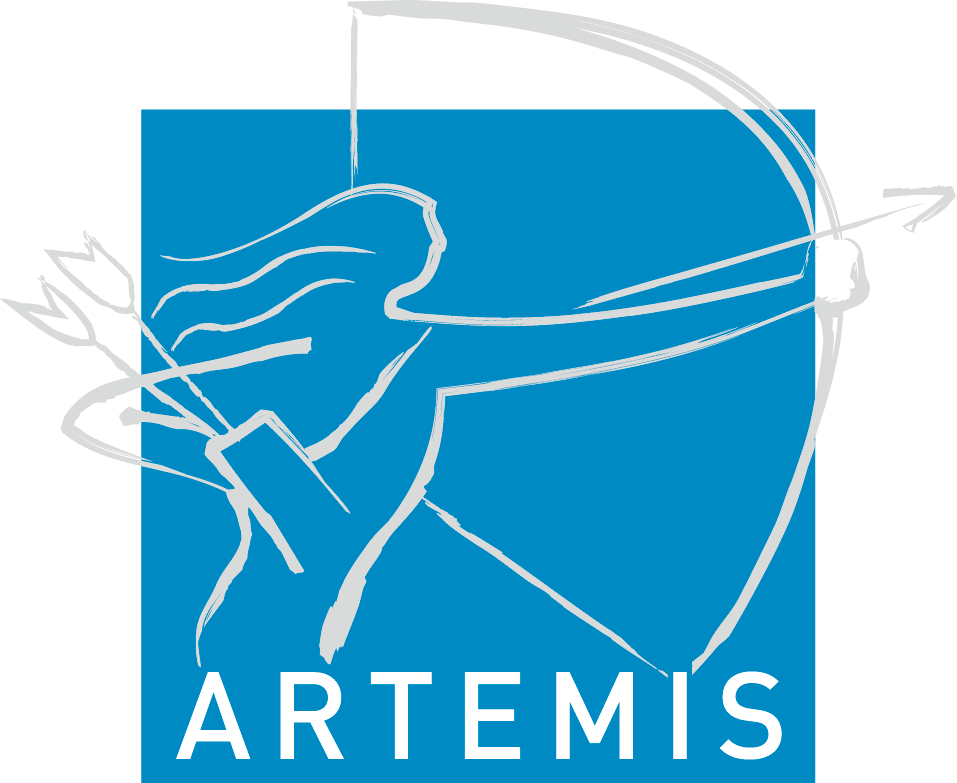
\includegraphics[width=2cm]{figures/artemis_logo}} & {ARTEMIS Innovation Pilot Project: Arrowhead\newline
%     THEME [SP1-JTI-ARTEMIS-2012-AIPP4 SP1-JTI-ARTEMIS-2012-AIPP6]\newline
%     [Production and Energy System Automation Intelligent-Built environment and urban infrastructure for sustainable and friendly cities]}
%   \end{tabularx}
%   \vspace*{-0.2cm}
 \end{center}

\newpage
%%

%% Table of Contents
\tableofcontents
\newpage
%%

\section{Overview}
\label{sec:overview}
This document describes the fundational principels for Eclispe
Arrowhead architecture and implementation platform. 


%\newpage

\subsection{Significant Prior Art}
\label{sec:prior_art}

Eclipse Arrowhead has its roots in service oriented arcitecture, SOA,
and its use for primarily far edge, edge and fog automation and
digitalsiation with interoperability to the cloud level.

A set of EU projects have built the foundation for whats now Eclipse
Arrowhead, current version 4.6.1 with the specifications for v5.0 in
the works. These projects are:
\begin{itemize}
\item Socrades
\item IMC-AESOP
\item Arrowhead
\item Productive4.0
\item Arrowhead Tools
\item AIMS5.0
\item Arrowhead fPVN
\end{itemize}

A couple of basic architectture ideas has been around since the prior
art projects:
\begin{itemize}
\item Socrades:
  \begin{itemize}
  \item Hard real time control using internet protocols
  \end{itemize}

\item IMC-AESOP:
  \begin{itemize}
  \item Objective to be capable of implementing real world SCADA and
    DCS systems.
  \item The local cloud concept was born. Local clouds are self
    contined for its intended operation enabling local security,
    protection and if equiped with TDMA network MAC real time
    properties can be achived.
  \item System are self contained for its intended operation,
    e.g. owning and responsible for its own data storage and compitational resources.

  \item Arrowhead:
    \begin{itemize}
    \item Objective to be interoperability to legacy and internet protocols and being
      Open Source.
    \item Basic SOA foundation established, Look-up, Late binding and
      Lossely coupled.
    \item Mandatory core systems defined: ServiceRegistry,
      Orcehstration, Authorisation
    \item Interoperability enabled through translation dynamically
      instatiated when needed.
    \item v3.3 released as open source      
    \end{itemize}
  
    \item Productive4.0:
      \begin{itemize}
      \item Arrowhead Framework becomes Eclipse Arrowhead architecture
        and implementation platform
      \item Extending the implementation platform - teh Arrowhead
        technology stack is defined
      \item v4.5 released
      \end{itemize}

      
    \item Arowheead Tools
      \begin{itemize}
      \item Objective to reduce engineereing cost with 20-50\%
      \item Extending the Eclipse Arrowehad technology stack
      \item v4.6 released
      \item Achived 30-95\%engineering cost and time reduction in 28
        industrial use cases along the extended IEC 81346 engineering process. 
      \end{itemize}
    \end{itemize}
\end{itemize}

In summary the industrial requirements setting hte scene for the
Eclipse Arrowhead developments comes from industiral automation and
digitalisation related to domains like e.g. automotive, aeronatics,
manufacturing, batch and continous processing, semiconductor
production, maintenance, buildings, energy, mining, logitics and smart
cities. The primary focus for the Eclispe Arrowhead SoS view is
integration and interoperability of edge and deep edge technology into
System of Systems with capabilites to connect to cloud e.g. for
data storage and high performance computing.    

 The current comprehensive high level architecture description of
 Eclipse Arrowhead architecture is the book ``IoT Automation -
 Arrowhead framework''  \cite{Delsing2017a}. The currently released
 core systems and associated documentations
 are avialable at \url{www.github.com/eclipsearrowhead}.

 \begin{figure}[ht!]
   \centering
   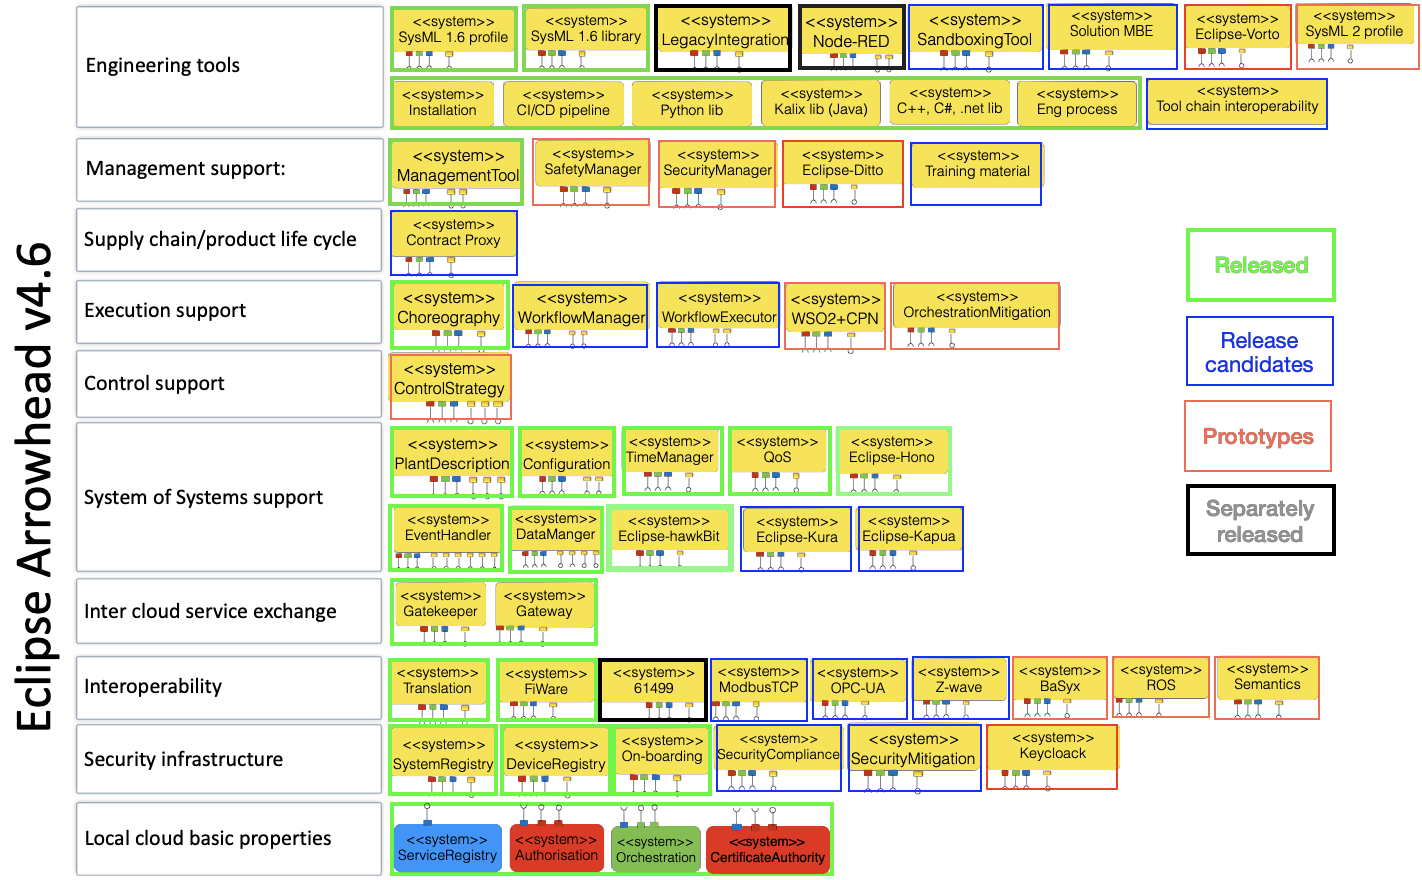
\includegraphics[width=0.9\linewidth]{figures/arrowhead_technology_stack}
   \caption{The Eclipse Arrowhead technology stack an dassoicated
     microsystems, released, relase candidates and protoypes.}
   \label{fig:technology_stack}
 \end{figure}

\subsection{Eclispe Arrowhead architecture philophosy}
\label{sec:use}

The architecture philiposy is based on the following key technology
decission and objectives:
\begin{itemize}
\item Key technology decisions
  \begin{itemize}
  \item A fully distributed microservice SOA approach shall be used
  \item Support for design and run time engineering

  \item A set of microsystems, the technology stack cf. Figure
    \ref{fig:technology_stack}, shall be provided. Use of one or many of
    these microsystems enables the implementation of automation and digitalisation solutions. 
    
    \begin{itemize}
    \item Three core microsystems considered as primary and almost
      mandatory, ServiceRegistry, Orcehstration, Authorisation,
      enabling Look-up, Late binding and Lossely coupling.
    \item A set of support microsystem will be defined and implemented
      covering the technology stack cf. Figure enabling implementation
      automation architectures like ISA-95 and RAMI4.0. 
      \ref{fig:technology_stack}.
      \end{itemize}

    \item Basic microsystem properties: A micosystem can be stateless
      or statefull. If statefull the microsystem is responsible for
      its own data stoarage perferable using a database and a well
      established/standardised datamodel.

    \item The local cloud concept shall be used providing segmentation
      and protection of functionall properties enabling differentieade
      security, safety, and real time properties within a solution
      architecture with managed access into a segment and between segements.

    \item Network technology agnostic, allowing for different network
      properties inside different local clouds.

    \item Documentation of the Eclipse Arrowhead architecture and
      solutions based thereon to follow the adopted documentation
      structure as shown in Figure \ref{fig:documentation_structure}.  
  
\begin{figure}[ht!]
   \centering
   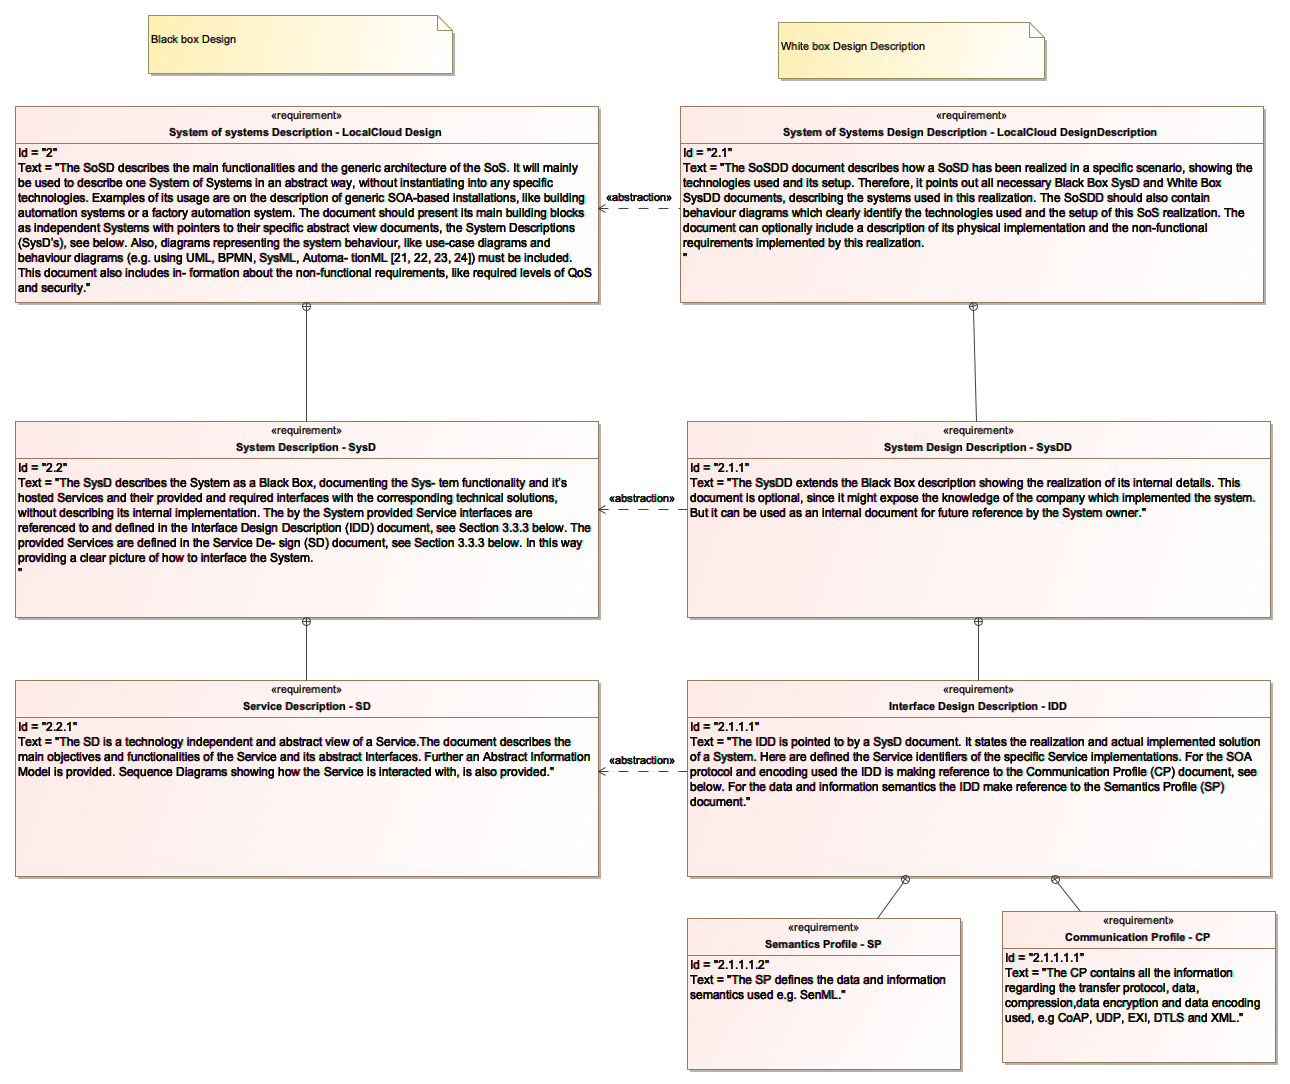
\includegraphics[width=0.9\linewidth]{figures/documentation_structure}
   \caption{The Eclipse Arrowhead documentation structure.}
   \label{fig:documentation_structure}
 \end{figure}


      
    \item Architectural levels defined are depicted in Figure \ref{fig:architecture_levels}.

    \end{itemize}

\begin{figure}[ht!]
   \centering
   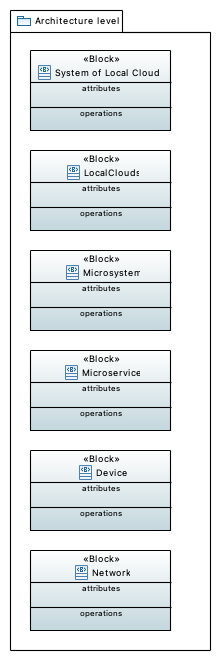
\includegraphics[height=14cm]{figures/ArrowheadArchitecturalLevels}
   \caption{The Eclipse Arrowhead architectural levels from network to
     System of Systems.}
   \label{fig:architecture_levels}
 \end{figure}


    
  \item Technology objectives: 
   \begin{itemize} 
      
    \item Interoperability support at Service level shall be provided
      regrding: SOA, IP and legacy protocols, encodings, compressions,
      security, data models, trough translators or dedicated
      adaptors. For data model interopeability between major standards
      like e.g. ISO10303, ISO 15926, IEC 81346 are prioritised.
      
    \item Security shall be supported at service exchange level with
      authentication, authorisation and audit. Security at finer
      granularity that service level is being addressed. Securityy is
      highly recommended but can be discarded if desired.  
      
    \item Secure on-boarding: On-boarding based on authentication of
      devices, microsystems and microservices shall be supproted.

    \item Support for multipe strategy direction. A strategy
      directions may be: Security, LifeCycle, Maintenance, Business,
      Audit, Monitoring, BusinessAdminstration, BusinessModels. This
      will also require ways of addressing interdependecies between
      the various stratgy directions.
    \item Model based engineering to support documentation,
      requirements validation, automated code generation and
      generation of deployment ready code packages (containers)
      \cite{Delsing2021a,Delsing2021b}

    \item Domain specific language based on UML/SysML \cite{Arrowhead_DSL}.
   
    \end{itemize}
    
  \end{itemize}

  

I set of terminologies used in the Eclipse Arrowhead devlopements and
supporting project are important to highlight. The following are
important to higlight since they may have different meaning in other
domains, contexts and projects. The document by Emanuel Palm and
Jerker Delsing has defined the most important vocabulary within the
Eclipse Arrowhead development \cite{Palm2023}. Some important updates
are:
\begin{itemize}
\item Service -$>$ Microservice
\item System -$>$ Microsystem

\end{itemize}

\begin{figure}[ht!]
   \centering
   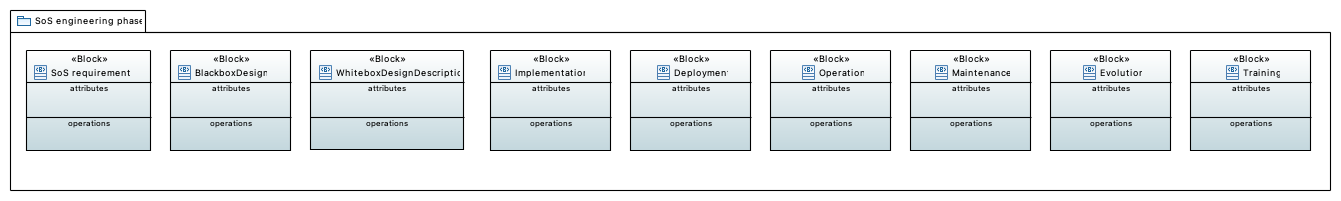
\includegraphics[width=0.9\linewidth]{figures/ArrowheadEngineeringProcess}
   \caption{The Eclipse Arrowhead engineering process is an extension
     of the IEC81346 engineering process.}
   \label{fig:engineering_process}
 \end{figure}


\section{Eclipse Arrowhead engineering process}
The Arrowhead engineering processs has primarly been documented in a
couple of papers by G. Urgese
et.al. \cite{Urgese2020,Urgese2022}, cf. Figure \ref{fig:engineering_process}. 

\begin{figure}[ht!]
   \centering
   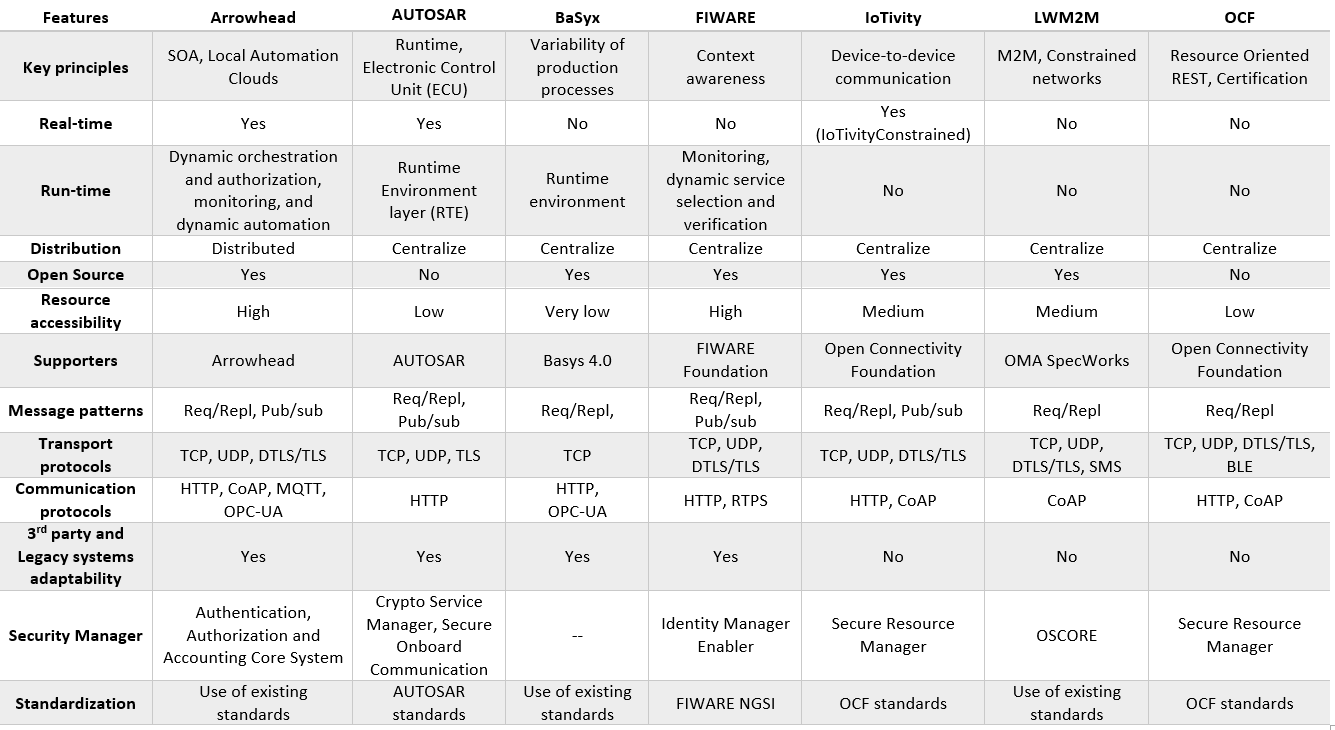
\includegraphics[width=0.9\linewidth]{figures/table}
   \caption{}
   \label{fig:IoT_framework_comparison}
 \end{figure}


\section{Comparison to other frameworks}
A recent comparison to other frameworks has been published by Cristina
Paniagua et.al \cite{Paniagua2021}. The summary table of this
comparison is reproduced in Figure \ref{fig:IoT_framework_comparison}.



\section{Implementation specifics}
For the current implementations a set of technologies has been choosen
for various reasons ranging from simple to use over ``this are the
technlogies I'm familiar to'' to ther are the technologies ``which
provides what I what''. Technologies used for implementations of
Eclipse Arrowhead microsystem are:

\begin{itemize}      
    \item Protocols: HTTP (REST), CoAP, MQTT, Websocket
    \item Network protocols: Ethernet, WiFi, 802.15.4
    \item Datamode standards used: SenML
    \item Security protocol: X.509 certificates and tokens, see \cite{Palm2022}
    \item Programing language: Java, Python
    \item Libraries: Java, C
    \item High performance: GO lang
\end{itemize}  
 





\bibliographystyle{IEEEtran}
\bibliography{arrowhead-bib}


\newpage

\section{Revision History}
\subsection{Amendments}

Revision history and Quality assurance as per examples below\color{black}

\noindent\begin{tabularx}{\textwidth}{| p{1cm} | p{3cm} | p{2cm} | X | p{4cm} |} \hline
\rowcolor{gray!33} No. & Date & Version & Subject of Amendments & Author \\ \hline

1 & 2023-05-08 & \arrowversion & & Jerker Delsing \\ \hline
2 & & & & \\ \hline
3 & & & & \\ \hline
\end{tabularx}

\subsection{Quality Assurance}

\noindent\begin{tabularx}{\textwidth}{| p{1cm} | p{3cm} | p{2cm} | X |} \hline
\rowcolor{gray!33} No. & Date & Version & Approved by \\ \hline

1 & 2022-01-10 & \arrowversion  &  \\ \hline

\end{tabularx}

\end{document}
%  LocalWords:  Arrowehad
